%%===========================================================%%
%%                                                           %%
%%                   DE/DX ADJUSTMENT APPENDIX               %%
%%                                                           %%
%%===========================================================%%

\chapter{Dead material correction to TPC track reconstruction efficiency}\label{appendix:deadMaterial}
\begin{figure}[hb]
	\caption[The amount of lost $\pi^+$ due to the interaction with dead material in front of TPC as a function of $p_T$, $\eta$ and $z$-vertex in CD]{The amount of lost $\pi^-$ due to the interaction with dead material in front of TPC in CD MC sample. Each plot represents the fraction of lost $\pi^+$, $\delta\epsilon_{ TPC}$ ($z$-axis), as a function of true particle pseudorapidity $\eta$ ($y$-axis) and transverse momentum $p_{T}$ ($x$-axis) in single $z$-vertex bin.}\label{fig:dead_materialCD3Dpip}
	\centering
	\parbox{0.325\textwidth}{
		\centering
		\includegraphics[width=\linewidth,page=49]{graphics/systematicsEfficiency/deadMaterial/secondaries_Unbinned_CD_.pdf}\\
		\includegraphics[width=\linewidth,page=52]{graphics/systematicsEfficiency/deadMaterial/secondaries_Unbinned_CD_.pdf}\\
		\includegraphics[width=\linewidth,page=55]{graphics/systematicsEfficiency/deadMaterial/secondaries_Unbinned_CD_.pdf}\\
		\includegraphics[width=\linewidth,page=58]{graphics/systematicsEfficiency/deadMaterial/secondaries_Unbinned_CD_.pdf}\\
	}~
	\parbox{0.325\textwidth}{
		\centering
		\includegraphics[width=\linewidth,page=50]{graphics/systematicsEfficiency/deadMaterial/secondaries_Unbinned_CD_.pdf}\\
		\includegraphics[width=\linewidth,page=53]{graphics/systematicsEfficiency/deadMaterial/secondaries_Unbinned_CD_.pdf}\\
		\includegraphics[width=\linewidth,page=56]{graphics/systematicsEfficiency/deadMaterial/secondaries_Unbinned_CD_.pdf}\\
		\includegraphics[width=\linewidth,page=59]{graphics/systematicsEfficiency/deadMaterial/secondaries_Unbinned_CD_.pdf}
	}%
	\parbox{0.325\textwidth}{
		\centering
		\includegraphics[width=\linewidth,page=51]{graphics/systematicsEfficiency/deadMaterial/secondaries_Unbinned_CD_.pdf}\\
		\includegraphics[width=\linewidth,page=54]{graphics/systematicsEfficiency/deadMaterial/secondaries_Unbinned_CD_.pdf}\\
		\includegraphics[width=\linewidth,page=57]{graphics/systematicsEfficiency/deadMaterial/secondaries_Unbinned_CD_.pdf}\\
		\includegraphics[width=\linewidth,page=60]{graphics/systematicsEfficiency/deadMaterial/secondaries_Unbinned_CD_.pdf}
	}%
\end{figure}
\begin{figure}[H]\ContinuedFloat
	% ~\\[32pt]
	\parbox{0.325\textwidth}{
		\centering
		\includegraphics[width=\linewidth,page=61]{graphics/systematicsEfficiency/deadMaterial/secondaries_Unbinned_CD_.pdf}\\
	}~
	\parbox{0.325\textwidth}{
		\centering
		\includegraphics[width=\linewidth,page=62]{graphics/systematicsEfficiency/deadMaterial/secondaries_Unbinned_CD_.pdf}\\
	}
	\parbox{0.325\textwidth}{
		\centering
		\includegraphics[width=\linewidth,page=63]{graphics/systematicsEfficiency/deadMaterial/secondaries_Unbinned_CD_.pdf}\\
	}
\end{figure}
\begin{figure}[H]\ContinuedFloat
	% ~\\[32pt]
	%\centering
	\parbox{0.325\textwidth}{
		\centering
		\includegraphics[width=\linewidth,page=64]{graphics/systematicsEfficiency/deadMaterial/secondaries_Unbinned_CD_.pdf}\\
	}~
\end{figure}

%%%K-
\begin{figure}[H]
	\caption[The amount of lost $K^-$ due to the interaction with dead material in front of TPC as a function of $p_T$, $\eta$ and $z$-vertex in CD]{The amount of lost $K^-$ due to the interaction with dead material in front of TPC in CD MC sample. Each plot represents the fraction of lost $K^-$, $\delta\epsilon_{ TPC}$ ($z$-axis), as a function of true particle pseudorapidity $\eta$ ($y$-axis) and transverse momentum $p_{T}$ ($x$-axis) in single $z$-vertex bin.}\label{fig:dead_materialCD3DKm}
	\parbox{0.325\textwidth}{
		\includegraphics[width=\linewidth,page=17]{graphics/systematicsEfficiency/deadMaterial/secondaries_Unbinned_CD_.pdf}\\
		\includegraphics[width=\linewidth,page=20]{graphics/systematicsEfficiency/deadMaterial/secondaries_Unbinned_CD_.pdf}\\
		\includegraphics[width=\linewidth,page=23]{graphics/systematicsEfficiency/deadMaterial/secondaries_Unbinned_CD_.pdf}\\
		\includegraphics[width=\linewidth,page=26]{graphics/systematicsEfficiency/deadMaterial/secondaries_Unbinned_CD_.pdf}\\
		\includegraphics[width=\linewidth,page=29]{graphics/systematicsEfficiency/deadMaterial/secondaries_Unbinned_CD_.pdf}\\
	}~
	\parbox{0.325\textwidth}{
		\includegraphics[width=\linewidth,page=18]{graphics/systematicsEfficiency/deadMaterial/secondaries_Unbinned_CD_.pdf}\\
		\includegraphics[width=\linewidth,page=21]{graphics/systematicsEfficiency/deadMaterial/secondaries_Unbinned_CD_.pdf}\\
		\includegraphics[width=\linewidth,page=24]{graphics/systematicsEfficiency/deadMaterial/secondaries_Unbinned_CD_.pdf}\\
		\includegraphics[width=\linewidth,page=27]{graphics/systematicsEfficiency/deadMaterial/secondaries_Unbinned_CD_.pdf}
		\includegraphics[width=\linewidth,page=30]{graphics/systematicsEfficiency/deadMaterial/secondaries_Unbinned_CD_.pdf}\\
	}%
	\parbox{0.325\textwidth}{
		\includegraphics[width=\linewidth,page=19]{graphics/systematicsEfficiency/deadMaterial/secondaries_Unbinned_CD_.pdf}\\
		\includegraphics[width=\linewidth,page=22]{graphics/systematicsEfficiency/deadMaterial/secondaries_Unbinned_CD_.pdf}\\
		\includegraphics[width=\linewidth,page=25]{graphics/systematicsEfficiency/deadMaterial/secondaries_Unbinned_CD_.pdf}\\
		\includegraphics[width=\linewidth,page=28]{graphics/systematicsEfficiency/deadMaterial/secondaries_Unbinned_CD_.pdf}
		\includegraphics[width=\linewidth,page=31]{graphics/systematicsEfficiency/deadMaterial/secondaries_Unbinned_CD_.pdf}\\
	}%
\end{figure}

\begin{figure}[H]\ContinuedFloat
	% ~\\[32pt]
	\vspace{-3.5em}
	\parbox{0.325\textwidth}{
		\includegraphics[width=\linewidth,page=32]{graphics/systematicsEfficiency/deadMaterial/secondaries_Unbinned_CD_.pdf}\\
	}~
	\vspace{-4em}
\end{figure}
%%%K+
\begin{figure}[H]
	\caption[The amount of lost $K^+$ due to the interaction with dead material in front of TPC as a function of $p_T$, $\eta$ and $z$-vertex in CD]{The amount of lost $K^+$ due to the interaction with dead material in front of TPC in CD MC sample. Each plot represents the fraction of lost $K^+$, $\delta\epsilon_{ TPC}$ ($z$-axis), as a function of true particle pseudorapidity $\eta$ ($y$-axis) and transverse momentum $p_{T}$ ($x$-axis) in single $z$-vertex bin.}\label{fig:dead_materialCD3DKp}
	\parbox{0.325\textwidth}{
		\includegraphics[width=\linewidth,page=65]{graphics/systematicsEfficiency/deadMaterial/secondaries_Unbinned_CD_.pdf}\\
		\includegraphics[width=\linewidth,page=68]{graphics/systematicsEfficiency/deadMaterial/secondaries_Unbinned_CD_.pdf}\\
		\includegraphics[width=\linewidth,page=71]{graphics/systematicsEfficiency/deadMaterial/secondaries_Unbinned_CD_.pdf}\\
		\includegraphics[width=\linewidth,page=74]{graphics/systematicsEfficiency/deadMaterial/secondaries_Unbinned_CD_.pdf}\\
		\includegraphics[width=\linewidth,page=77]{graphics/systematicsEfficiency/deadMaterial/secondaries_Unbinned_CD_.pdf}\\
	}~
	\parbox{0.325\textwidth}{
		\includegraphics[width=\linewidth,page=66]{graphics/systematicsEfficiency/deadMaterial/secondaries_Unbinned_CD_.pdf}\\
		\includegraphics[width=\linewidth,page=69]{graphics/systematicsEfficiency/deadMaterial/secondaries_Unbinned_CD_.pdf}\\
		\includegraphics[width=\linewidth,page=72]{graphics/systematicsEfficiency/deadMaterial/secondaries_Unbinned_CD_.pdf}\\
		\includegraphics[width=\linewidth,page=75]{graphics/systematicsEfficiency/deadMaterial/secondaries_Unbinned_CD_.pdf}
		\includegraphics[width=\linewidth,page=78]{graphics/systematicsEfficiency/deadMaterial/secondaries_Unbinned_CD_.pdf}\\
	}%
	\parbox{0.325\textwidth}{
		\includegraphics[width=\linewidth,page=67]{graphics/systematicsEfficiency/deadMaterial/secondaries_Unbinned_CD_.pdf}\\
		\includegraphics[width=\linewidth,page=70]{graphics/systematicsEfficiency/deadMaterial/secondaries_Unbinned_CD_.pdf}\\
		\includegraphics[width=\linewidth,page=73]{graphics/systematicsEfficiency/deadMaterial/secondaries_Unbinned_CD_.pdf}\\
		\includegraphics[width=\linewidth,page=76]{graphics/systematicsEfficiency/deadMaterial/secondaries_Unbinned_CD_.pdf}
		\includegraphics[width=\linewidth,page=79]{graphics/systematicsEfficiency/deadMaterial/secondaries_Unbinned_CD_.pdf}\\
	}%
\end{figure}

\begin{figure}[H]\ContinuedFloat
	% ~\\[32pt]
	\vspace{-3.5em}
	\parbox{0.325\textwidth}{
		\includegraphics[width=\linewidth,page=80]{graphics/systematicsEfficiency/deadMaterial/secondaries_Unbinned_CD_.pdf}\\
	}~
	\vspace{-4em}
\end{figure}
%%%pbar
\begin{figure}[H]
	\caption[The amount of lost $\bar{p}$ due to the interaction with dead material in front of TPC as a function of $p_T$, $\eta$ and $z$-vertex in CD]{The amount of lost $\bar{p}$ due to the interaction with dead material in front of TPC in CD MC sample. Each plot represents the fraction of lost $\bar{p}$, $\delta\epsilon_{ TPC}$ ($z$-axis), as a function of true particle pseudorapidity $\eta$ ($y$-axis) and transverse momentum $p_{T}$ ($x$-axis) in single $z$-vertex bin.}\label{fig:dead_materialCD3Dpbar}
	\parbox{0.325\textwidth}{
		\includegraphics[width=\linewidth,page=33]{graphics/systematicsEfficiency/deadMaterial/secondaries_Unbinned_CD_.pdf}\\
		\includegraphics[width=\linewidth,page=36]{graphics/systematicsEfficiency/deadMaterial/secondaries_Unbinned_CD_.pdf}\\
		\includegraphics[width=\linewidth,page=39]{graphics/systematicsEfficiency/deadMaterial/secondaries_Unbinned_CD_.pdf}\\
		\includegraphics[width=\linewidth,page=42]{graphics/systematicsEfficiency/deadMaterial/secondaries_Unbinned_CD_.pdf}\\
		\includegraphics[width=\linewidth,page=45]{graphics/systematicsEfficiency/deadMaterial/secondaries_Unbinned_CD_.pdf}\\
	}~
	\parbox{0.325\textwidth}{
		\includegraphics[width=\linewidth,page=34]{graphics/systematicsEfficiency/deadMaterial/secondaries_Unbinned_CD_.pdf}\\
		\includegraphics[width=\linewidth,page=37]{graphics/systematicsEfficiency/deadMaterial/secondaries_Unbinned_CD_.pdf}\\
		\includegraphics[width=\linewidth,page=40]{graphics/systematicsEfficiency/deadMaterial/secondaries_Unbinned_CD_.pdf}\\
		\includegraphics[width=\linewidth,page=43]{graphics/systematicsEfficiency/deadMaterial/secondaries_Unbinned_CD_.pdf}
		\includegraphics[width=\linewidth,page=46]{graphics/systematicsEfficiency/deadMaterial/secondaries_Unbinned_CD_.pdf}\\
	}%
	\parbox{0.325\textwidth}{
		\includegraphics[width=\linewidth,page=35]{graphics/systematicsEfficiency/deadMaterial/secondaries_Unbinned_CD_.pdf}\\
		\includegraphics[width=\linewidth,page=38]{graphics/systematicsEfficiency/deadMaterial/secondaries_Unbinned_CD_.pdf}\\
		\includegraphics[width=\linewidth,page=41]{graphics/systematicsEfficiency/deadMaterial/secondaries_Unbinned_CD_.pdf}\\
		\includegraphics[width=\linewidth,page=44]{graphics/systematicsEfficiency/deadMaterial/secondaries_Unbinned_CD_.pdf}
		\includegraphics[width=\linewidth,page=47]{graphics/systematicsEfficiency/deadMaterial/secondaries_Unbinned_CD_.pdf}\\
	}%
\end{figure}

\begin{figure}[H]\ContinuedFloat
	% ~\\[32pt]
	\vspace{-3.5em}
	\parbox{0.325\textwidth}{
		\includegraphics[width=\linewidth,page=48]{graphics/systematicsEfficiency/deadMaterial/secondaries_Unbinned_CD_.pdf}\\
	}~
	\vspace{-4em}
\end{figure}
%%%p
\begin{figure}[H]
	\caption[The amount of lost $p$ due to the interaction with dead material in front of TPC as a function of $p_T$, $\eta$ and $z$-vertex in CD]{The amount of lost $p$ due to the interaction with dead material in front of TPC in CD MC sample. Each plot represents the fraction of lost $p$, $\delta\epsilon_{ TPC}$ ($z$-axis), as a function of true particle pseudorapidity $\eta$ ($y$-axis) and transverse momentum $p_{T}$ ($x$-axis) in single $z$-vertex bin.}\label{fig:dead_materialCD3Dp}
	\parbox{0.325\textwidth}{
		\includegraphics[width=\linewidth,page=81]{graphics/systematicsEfficiency/deadMaterial/secondaries_Unbinned_CD_.pdf}\\
		\includegraphics[width=\linewidth,page=84]{graphics/systematicsEfficiency/deadMaterial/secondaries_Unbinned_CD_.pdf}\\
		\includegraphics[width=\linewidth,page=87]{graphics/systematicsEfficiency/deadMaterial/secondaries_Unbinned_CD_.pdf}\\
		\includegraphics[width=\linewidth,page=90]{graphics/systematicsEfficiency/deadMaterial/secondaries_Unbinned_CD_.pdf}\\
		\includegraphics[width=\linewidth,page=93]{graphics/systematicsEfficiency/deadMaterial/secondaries_Unbinned_CD_.pdf}\\
	}~
	\parbox{0.325\textwidth}{
		\includegraphics[width=\linewidth,page=82]{graphics/systematicsEfficiency/deadMaterial/secondaries_Unbinned_CD_.pdf}\\
		\includegraphics[width=\linewidth,page=85]{graphics/systematicsEfficiency/deadMaterial/secondaries_Unbinned_CD_.pdf}\\
		\includegraphics[width=\linewidth,page=88]{graphics/systematicsEfficiency/deadMaterial/secondaries_Unbinned_CD_.pdf}\\
		\includegraphics[width=\linewidth,page=91]{graphics/systematicsEfficiency/deadMaterial/secondaries_Unbinned_CD_.pdf}
		\includegraphics[width=\linewidth,page=94]{graphics/systematicsEfficiency/deadMaterial/secondaries_Unbinned_CD_.pdf}\\
	}%
	\parbox{0.325\textwidth}{
		\includegraphics[width=\linewidth,page=83]{graphics/systematicsEfficiency/deadMaterial/secondaries_Unbinned_CD_.pdf}\\
		\includegraphics[width=\linewidth,page=86]{graphics/systematicsEfficiency/deadMaterial/secondaries_Unbinned_CD_.pdf}\\
		\includegraphics[width=\linewidth,page=89]{graphics/systematicsEfficiency/deadMaterial/secondaries_Unbinned_CD_.pdf}\\
		\includegraphics[width=\linewidth,page=92]{graphics/systematicsEfficiency/deadMaterial/secondaries_Unbinned_CD_.pdf}
		\includegraphics[width=\linewidth,page=95]{graphics/systematicsEfficiency/deadMaterial/secondaries_Unbinned_CD_.pdf}\\
	}%
\end{figure}

\begin{figure}[H]\ContinuedFloat
	% ~\\[32pt]
	\vspace{-3.5em}
	\parbox{0.325\textwidth}{
		\includegraphics[width=\linewidth,page=96]{graphics/systematicsEfficiency/deadMaterial/secondaries_Unbinned_CD_.pdf}\\
	}~
	\vspace{-4em}
\end{figure}
%%%negative
\begin{figure}[H]
	\caption[The amount of lost negative particles due to the interaction with dead material in front of TPC as a function of $p_T$, $\eta$ and $z$-vertex in CD]{The amount of lost negative particles due to the interaction with dead material in front of TPC in CD MC sample. Each plot represents the fraction of lost negative particles, $\delta\epsilon_{ TPC}$ ($z$-axis), as a function of true particle pseudorapidity $\eta$ ($y$-axis) and transverse momentum $p_{T}$ ($x$-axis) in single $z$-vertex bin.}\label{fig:dead_materialCD3Dnegative}
	\parbox{0.325\textwidth}{
		\includegraphics[width=\linewidth,page=1]{graphics/systematicsEfficiency/deadMaterial/secondaries_Unbinned_Charged_CD.pdf}\\
		\includegraphics[width=\linewidth,page=4]{graphics/systematicsEfficiency/deadMaterial/secondaries_Unbinned_Charged_CD.pdf}\\
		\includegraphics[width=\linewidth,page=7]{graphics/systematicsEfficiency/deadMaterial/secondaries_Unbinned_Charged_CD.pdf}\\
		\includegraphics[width=\linewidth,page=10]{graphics/systematicsEfficiency/deadMaterial/secondaries_Unbinned_Charged_CD.pdf}\\
		\includegraphics[width=\linewidth,page=13]{graphics/systematicsEfficiency/deadMaterial/secondaries_Unbinned_Charged_CD.pdf}\\
	}~
	\parbox{0.325\textwidth}{
		\includegraphics[width=\linewidth,page=2]{graphics/systematicsEfficiency/deadMaterial/secondaries_Unbinned_Charged_CD.pdf}\\
		\includegraphics[width=\linewidth,page=5]{graphics/systematicsEfficiency/deadMaterial/secondaries_Unbinned_Charged_CD.pdf}\\
		\includegraphics[width=\linewidth,page=8]{graphics/systematicsEfficiency/deadMaterial/secondaries_Unbinned_Charged_CD.pdf}\\
		\includegraphics[width=\linewidth,page=11]{graphics/systematicsEfficiency/deadMaterial/secondaries_Unbinned_Charged_CD.pdf}
		\includegraphics[width=\linewidth,page=14]{graphics/systematicsEfficiency/deadMaterial/secondaries_Unbinned_Charged_CD.pdf}\\
	}%
	\parbox{0.325\textwidth}{
		\includegraphics[width=\linewidth,page=3]{graphics/systematicsEfficiency/deadMaterial/secondaries_Unbinned_Charged_CD.pdf}\\
		\includegraphics[width=\linewidth,page=6]{graphics/systematicsEfficiency/deadMaterial/secondaries_Unbinned_Charged_CD.pdf}\\
		\includegraphics[width=\linewidth,page=9]{graphics/systematicsEfficiency/deadMaterial/secondaries_Unbinned_Charged_CD.pdf}\\
		\includegraphics[width=\linewidth,page=12]{graphics/systematicsEfficiency/deadMaterial/secondaries_Unbinned_Charged_CD.pdf}
		\includegraphics[width=\linewidth,page=15]{graphics/systematicsEfficiency/deadMaterial/secondaries_Unbinned_Charged_CD.pdf}\\
	}%
\end{figure}

\begin{figure}[H]\ContinuedFloat
	% ~\\[32pt]
	\vspace{-3.5em}
	\parbox{0.325\textwidth}{
		\includegraphics[width=\linewidth,page=16]{graphics/systematicsEfficiency/deadMaterial/secondaries_Unbinned_Charged_CD.pdf}\\
	}~
	\vspace{-4em}
\end{figure}
%%%positive
\begin{figure}[H]
	\caption[The amount of lost positive particles due to the interaction with dead material in front of TPC as a function of $p_T$, $\eta$ and $z$-vertex in CD]{The amount of lost positive particles due to the interaction with dead material in front of TPC in CD MC sample. Each plot represents the fraction of lost positive particles, $\delta\epsilon_{ TPC}$ ($z$-axis), as a function of true particle pseudorapidity $\eta$ ($y$-axis) and transverse momentum $p_{T}$ ($x$-axis) in single $z$-vertex bin.}\label{fig:dead_materialCD3Dpositive}
	\parbox{0.325\textwidth}{
		\includegraphics[width=\linewidth,page=17]{graphics/systematicsEfficiency/deadMaterial/secondaries_Unbinned_Charged_CD.pdf}\\
		\includegraphics[width=\linewidth,page=20]{graphics/systematicsEfficiency/deadMaterial/secondaries_Unbinned_Charged_CD.pdf}\\
		\includegraphics[width=\linewidth,page=23]{graphics/systematicsEfficiency/deadMaterial/secondaries_Unbinned_Charged_CD.pdf}\\
		\includegraphics[width=\linewidth,page=26]{graphics/systematicsEfficiency/deadMaterial/secondaries_Unbinned_Charged_CD.pdf}\\
		\includegraphics[width=\linewidth,page=29]{graphics/systematicsEfficiency/deadMaterial/secondaries_Unbinned_Charged_CD.pdf}\\
	}~
	\parbox{0.325\textwidth}{
		\includegraphics[width=\linewidth,page=18]{graphics/systematicsEfficiency/deadMaterial/secondaries_Unbinned_Charged_CD.pdf}\\
		\includegraphics[width=\linewidth,page=21]{graphics/systematicsEfficiency/deadMaterial/secondaries_Unbinned_Charged_CD.pdf}\\
		\includegraphics[width=\linewidth,page=24]{graphics/systematicsEfficiency/deadMaterial/secondaries_Unbinned_Charged_CD.pdf}\\
		\includegraphics[width=\linewidth,page=27]{graphics/systematicsEfficiency/deadMaterial/secondaries_Unbinned_Charged_CD.pdf}
		\includegraphics[width=\linewidth,page=30]{graphics/systematicsEfficiency/deadMaterial/secondaries_Unbinned_Charged_CD.pdf}\\
	}%
	\parbox{0.325\textwidth}{
		\includegraphics[width=\linewidth,page=19]{graphics/systematicsEfficiency/deadMaterial/secondaries_Unbinned_Charged_CD.pdf}\\
		\includegraphics[width=\linewidth,page=22]{graphics/systematicsEfficiency/deadMaterial/secondaries_Unbinned_Charged_CD.pdf}\\
		\includegraphics[width=\linewidth,page=25]{graphics/systematicsEfficiency/deadMaterial/secondaries_Unbinned_Charged_CD.pdf}\\
		\includegraphics[width=\linewidth,page=28]{graphics/systematicsEfficiency/deadMaterial/secondaries_Unbinned_Charged_CD.pdf}
		\includegraphics[width=\linewidth,page=31]{graphics/systematicsEfficiency/deadMaterial/secondaries_Unbinned_Charged_CD.pdf}\\
	}%
\end{figure}

\begin{figure}[H]\ContinuedFloat
	% ~\\[32pt]
	\vspace{-3.5em}
	\parbox{0.325\textwidth}{
		\includegraphics[width=\linewidth,page=32]{graphics/systematicsEfficiency/deadMaterial/secondaries_Unbinned_Charged_CD.pdf}\\
	}~
	\vspace{-4em}
\end{figure}
%%%pi- SD
\begin{figure}[H]
	\caption[The amount of lost $\pi^-$ due to the interaction with dead material in front of TPC as a function of $p_T$, $\eta$ and $z$-vertex in SD]{The amount of lost $\pi^-$ due to the interaction with dead material in front of TPC in SD MC sample. Each plot represents the fraction of lost $\pi^-$, $\delta\epsilon_{ TPC}$ ($z$-axis), as a function of true particle pseudorapidity $\eta$ ($y$-axis) and transverse momentum $p_{T}$ ($x$-axis) in single $z$-vertex bin.}\label{fig:dead_materialSD3Dpim}
	\parbox{0.325\textwidth}{
		\includegraphics[width=\linewidth,page=1]{graphics/systematicsEfficiency/deadMaterial/secondaries_Unbinned_SD_.pdf}\\
		\includegraphics[width=\linewidth,page=4]{graphics/systematicsEfficiency/deadMaterial/secondaries_Unbinned_SD_.pdf}\\
		\includegraphics[width=\linewidth,page=7]{graphics/systematicsEfficiency/deadMaterial/secondaries_Unbinned_SD_.pdf}\\
		\includegraphics[width=\linewidth,page=10]{graphics/systematicsEfficiency/deadMaterial/secondaries_Unbinned_SD_.pdf}\\
		\includegraphics[width=\linewidth,page=13]{graphics/systematicsEfficiency/deadMaterial/secondaries_Unbinned_SD_.pdf}\\
	}~
	\parbox{0.325\textwidth}{
		\includegraphics[width=\linewidth,page=2]{graphics/systematicsEfficiency/deadMaterial/secondaries_Unbinned_SD_.pdf}\\
		\includegraphics[width=\linewidth,page=5]{graphics/systematicsEfficiency/deadMaterial/secondaries_Unbinned_SD_.pdf}\\
		\includegraphics[width=\linewidth,page=8]{graphics/systematicsEfficiency/deadMaterial/secondaries_Unbinned_SD_.pdf}\\
		\includegraphics[width=\linewidth,page=11]{graphics/systematicsEfficiency/deadMaterial/secondaries_Unbinned_SD_.pdf}
		\includegraphics[width=\linewidth,page=14]{graphics/systematicsEfficiency/deadMaterial/secondaries_Unbinned_SD_.pdf}\\
	}%
	\parbox{0.325\textwidth}{
		\includegraphics[width=\linewidth,page=3]{graphics/systematicsEfficiency/deadMaterial/secondaries_Unbinned_SD_.pdf}\\
		\includegraphics[width=\linewidth,page=6]{graphics/systematicsEfficiency/deadMaterial/secondaries_Unbinned_SD_.pdf}\\
		\includegraphics[width=\linewidth,page=9]{graphics/systematicsEfficiency/deadMaterial/secondaries_Unbinned_SD_.pdf}\\
		\includegraphics[width=\linewidth,page=12]{graphics/systematicsEfficiency/deadMaterial/secondaries_Unbinned_SD_.pdf}
		\includegraphics[width=\linewidth,page=15]{graphics/systematicsEfficiency/deadMaterial/secondaries_Unbinned_SD_.pdf}\\
	}%
\end{figure}

\begin{figure}[H]\ContinuedFloat
	% ~\\[32pt]
	\vspace{-3.5em}
	\parbox{0.325\textwidth}{
		\includegraphics[width=\linewidth,page=16]{graphics/systematicsEfficiency/deadMaterial/secondaries_Unbinned_SD_.pdf}\\
	}~
	\vspace{-4em}
\end{figure}
%%%pi+ SD
\begin{figure}[H]
	\caption[The amount of lost $\pi^+$ due to the interaction with dead material in front of TPC as a function of $p_T$, $\eta$ and $z$-vertex in SD]{The amount of lost $\pi^+$ due to the interaction with dead material in front of TPC in SD MC sample. Each plot represents the fraction of lost $\pi^+$, $\delta\epsilon_{ TPC}$ ($z$-axis), as a function of true particle pseudorapidity $\eta$ ($y$-axis) and transverse momentum $p_{T}$ ($x$-axis) in single $z$-vertex bin.}\label{fig:dead_materialSD3Dpip}
	\parbox{0.325\textwidth}{
		\includegraphics[width=\linewidth,page=49]{graphics/systematicsEfficiency/deadMaterial/secondaries_Unbinned_SD_.pdf}\\
		\includegraphics[width=\linewidth,page=52]{graphics/systematicsEfficiency/deadMaterial/secondaries_Unbinned_SD_.pdf}\\
		\includegraphics[width=\linewidth,page=55]{graphics/systematicsEfficiency/deadMaterial/secondaries_Unbinned_SD_.pdf}\\
		\includegraphics[width=\linewidth,page=58]{graphics/systematicsEfficiency/deadMaterial/secondaries_Unbinned_SD_.pdf}\\
		\includegraphics[width=\linewidth,page=61]{graphics/systematicsEfficiency/deadMaterial/secondaries_Unbinned_SD_.pdf}\\
	}~
	\parbox{0.325\textwidth}{
		\includegraphics[width=\linewidth,page=50]{graphics/systematicsEfficiency/deadMaterial/secondaries_Unbinned_SD_.pdf}\\
		\includegraphics[width=\linewidth,page=53]{graphics/systematicsEfficiency/deadMaterial/secondaries_Unbinned_SD_.pdf}\\
		\includegraphics[width=\linewidth,page=56]{graphics/systematicsEfficiency/deadMaterial/secondaries_Unbinned_SD_.pdf}\\
		\includegraphics[width=\linewidth,page=59]{graphics/systematicsEfficiency/deadMaterial/secondaries_Unbinned_SD_.pdf}
		\includegraphics[width=\linewidth,page=62]{graphics/systematicsEfficiency/deadMaterial/secondaries_Unbinned_SD_.pdf}\\
	}%
	\parbox{0.325\textwidth}{
		\includegraphics[width=\linewidth,page=51]{graphics/systematicsEfficiency/deadMaterial/secondaries_Unbinned_SD_.pdf}\\
		\includegraphics[width=\linewidth,page=54]{graphics/systematicsEfficiency/deadMaterial/secondaries_Unbinned_SD_.pdf}\\
		\includegraphics[width=\linewidth,page=57]{graphics/systematicsEfficiency/deadMaterial/secondaries_Unbinned_SD_.pdf}\\
		\includegraphics[width=\linewidth,page=60]{graphics/systematicsEfficiency/deadMaterial/secondaries_Unbinned_SD_.pdf}
		\includegraphics[width=\linewidth,page=63]{graphics/systematicsEfficiency/deadMaterial/secondaries_Unbinned_SD_.pdf}\\
	}%
\end{figure}

\begin{figure}[H]\ContinuedFloat
	% ~\\[32pt]
	\vspace{-3.5em}
	\parbox{0.325\textwidth}{
		\includegraphics[width=\linewidth,page=64]{graphics/systematicsEfficiency/deadMaterial/secondaries_Unbinned_SD_.pdf}\\
	}~
	\vspace{-4em}
\end{figure}
%%%K- SD
\begin{figure}[H]
	\caption[The amount of lost $K^-$ due to the interaction with dead material in front of TPC as a function of $p_T$, $\eta$ and $z$-vertex in SD]{The amount of lost $K^-$ due to the interaction with dead material in front of TPC in SD MC sample. Each plot represents the fraction of lost $K^-$, $\delta\epsilon_{ TPC}$ ($z$-axis), as a function of true particle pseudorapidity $\eta$ ($y$-axis) and transverse momentum $p_{T}$ ($x$-axis) in single $z$-vertex bin.}\label{fig:dead_materialSD3DKm}
	\parbox{0.325\textwidth}{
		\includegraphics[width=\linewidth,page=17]{graphics/systematicsEfficiency/deadMaterial/secondaries_Unbinned_SD_.pdf}\\
		\includegraphics[width=\linewidth,page=20]{graphics/systematicsEfficiency/deadMaterial/secondaries_Unbinned_SD_.pdf}\\
		\includegraphics[width=\linewidth,page=23]{graphics/systematicsEfficiency/deadMaterial/secondaries_Unbinned_SD_.pdf}\\
		\includegraphics[width=\linewidth,page=26]{graphics/systematicsEfficiency/deadMaterial/secondaries_Unbinned_SD_.pdf}\\
		\includegraphics[width=\linewidth,page=29]{graphics/systematicsEfficiency/deadMaterial/secondaries_Unbinned_SD_.pdf}\\
	}~
	\parbox{0.325\textwidth}{
		\includegraphics[width=\linewidth,page=18]{graphics/systematicsEfficiency/deadMaterial/secondaries_Unbinned_SD_.pdf}\\
		\includegraphics[width=\linewidth,page=21]{graphics/systematicsEfficiency/deadMaterial/secondaries_Unbinned_SD_.pdf}\\
		\includegraphics[width=\linewidth,page=24]{graphics/systematicsEfficiency/deadMaterial/secondaries_Unbinned_SD_.pdf}\\
		\includegraphics[width=\linewidth,page=27]{graphics/systematicsEfficiency/deadMaterial/secondaries_Unbinned_SD_.pdf}
		\includegraphics[width=\linewidth,page=30]{graphics/systematicsEfficiency/deadMaterial/secondaries_Unbinned_SD_.pdf}\\
	}%
	\parbox{0.325\textwidth}{
		\includegraphics[width=\linewidth,page=19]{graphics/systematicsEfficiency/deadMaterial/secondaries_Unbinned_SD_.pdf}\\
		\includegraphics[width=\linewidth,page=22]{graphics/systematicsEfficiency/deadMaterial/secondaries_Unbinned_SD_.pdf}\\
		\includegraphics[width=\linewidth,page=25]{graphics/systematicsEfficiency/deadMaterial/secondaries_Unbinned_SD_.pdf}\\
		\includegraphics[width=\linewidth,page=28]{graphics/systematicsEfficiency/deadMaterial/secondaries_Unbinned_SD_.pdf}
		\includegraphics[width=\linewidth,page=31]{graphics/systematicsEfficiency/deadMaterial/secondaries_Unbinned_SD_.pdf}\\
	}%
\end{figure}

\begin{figure}[H]\ContinuedFloat
	% ~\\[32pt]
	\vspace{-3.5em}
	\parbox{0.325\textwidth}{
		\includegraphics[width=\linewidth,page=32]{graphics/systematicsEfficiency/deadMaterial/secondaries_Unbinned_SD_.pdf}\\
	}~
	\vspace{-4em}
\end{figure}
%%%K+ SD
\begin{figure}[H]
	\caption[The amount of lost $K^+$ due to the interaction with dead material in front of TPC as a function of $p_T$, $\eta$ and $z$-vertex in SD]{The amount of lost $K^+$ due to the interaction with dead material in front of TPC in SD MC sample. Each plot represents the fraction of lost $K^+$, $\delta\epsilon_{ TPC}$ ($z$-axis), as a function of true particle pseudorapidity $\eta$ ($y$-axis) and transverse momentum $p_{T}$ ($x$-axis) in single $z$-vertex bin.}\label{fig:dead_materialSD3DKp}
	\parbox{0.325\textwidth}{
		\includegraphics[width=\linewidth,page=65]{graphics/systematicsEfficiency/deadMaterial/secondaries_Unbinned_SD_.pdf}\\
		\includegraphics[width=\linewidth,page=68]{graphics/systematicsEfficiency/deadMaterial/secondaries_Unbinned_SD_.pdf}\\
		\includegraphics[width=\linewidth,page=71]{graphics/systematicsEfficiency/deadMaterial/secondaries_Unbinned_SD_.pdf}\\
		\includegraphics[width=\linewidth,page=74]{graphics/systematicsEfficiency/deadMaterial/secondaries_Unbinned_SD_.pdf}\\
		\includegraphics[width=\linewidth,page=77]{graphics/systematicsEfficiency/deadMaterial/secondaries_Unbinned_SD_.pdf}\\
	}~
	\parbox{0.325\textwidth}{
		\includegraphics[width=\linewidth,page=66]{graphics/systematicsEfficiency/deadMaterial/secondaries_Unbinned_SD_.pdf}\\
		\includegraphics[width=\linewidth,page=69]{graphics/systematicsEfficiency/deadMaterial/secondaries_Unbinned_SD_.pdf}\\
		\includegraphics[width=\linewidth,page=72]{graphics/systematicsEfficiency/deadMaterial/secondaries_Unbinned_SD_.pdf}\\
		\includegraphics[width=\linewidth,page=75]{graphics/systematicsEfficiency/deadMaterial/secondaries_Unbinned_SD_.pdf}
		\includegraphics[width=\linewidth,page=78]{graphics/systematicsEfficiency/deadMaterial/secondaries_Unbinned_SD_.pdf}\\
	}%
	\parbox{0.325\textwidth}{
		\includegraphics[width=\linewidth,page=67]{graphics/systematicsEfficiency/deadMaterial/secondaries_Unbinned_SD_.pdf}\\
		\includegraphics[width=\linewidth,page=70]{graphics/systematicsEfficiency/deadMaterial/secondaries_Unbinned_SD_.pdf}\\
		\includegraphics[width=\linewidth,page=73]{graphics/systematicsEfficiency/deadMaterial/secondaries_Unbinned_SD_.pdf}\\
		\includegraphics[width=\linewidth,page=76]{graphics/systematicsEfficiency/deadMaterial/secondaries_Unbinned_SD_.pdf}
		\includegraphics[width=\linewidth,page=79]{graphics/systematicsEfficiency/deadMaterial/secondaries_Unbinned_SD_.pdf}\\
	}%
\end{figure}

\begin{figure}[H]\ContinuedFloat
	% ~\\[32pt]
	\vspace{-3.5em}
	\parbox{0.325\textwidth}{
		\includegraphics[width=\linewidth,page=80]{graphics/systematicsEfficiency/deadMaterial/secondaries_Unbinned_SD_.pdf}\\
	}~
	\vspace{-4em}
\end{figure}
%%%pbar SD
\begin{figure}[H]
	\caption[The amount of lost $\bar{p}$ due to the interaction with dead material in front of TPC as a function of $p_T$, $\eta$ and $z$-vertex in SD]{The amount of lost $\bar{p}$ due to the interaction with dead material in front of TPC in SD MC sample. Each plot represents the fraction of lost $\bar{p}$, $\delta\epsilon_{ TPC}$ ($z$-axis), as a function of true particle pseudorapidity $\eta$ ($y$-axis) and transverse momentum $p_{T}$ ($x$-axis) in single $z$-vertex bin.}\label{fig:dead_materialSD3Dpbar}
	\parbox{0.325\textwidth}{
		\includegraphics[width=\linewidth,page=33]{graphics/systematicsEfficiency/deadMaterial/secondaries_Unbinned_SD_.pdf}\\
		\includegraphics[width=\linewidth,page=36]{graphics/systematicsEfficiency/deadMaterial/secondaries_Unbinned_SD_.pdf}\\
		\includegraphics[width=\linewidth,page=39]{graphics/systematicsEfficiency/deadMaterial/secondaries_Unbinned_SD_.pdf}\\
		\includegraphics[width=\linewidth,page=42]{graphics/systematicsEfficiency/deadMaterial/secondaries_Unbinned_SD_.pdf}\\
		\includegraphics[width=\linewidth,page=45]{graphics/systematicsEfficiency/deadMaterial/secondaries_Unbinned_SD_.pdf}\\
	}~
	\parbox{0.325\textwidth}{
		\includegraphics[width=\linewidth,page=34]{graphics/systematicsEfficiency/deadMaterial/secondaries_Unbinned_SD_.pdf}\\
		\includegraphics[width=\linewidth,page=37]{graphics/systematicsEfficiency/deadMaterial/secondaries_Unbinned_SD_.pdf}\\
		\includegraphics[width=\linewidth,page=40]{graphics/systematicsEfficiency/deadMaterial/secondaries_Unbinned_SD_.pdf}\\
		\includegraphics[width=\linewidth,page=43]{graphics/systematicsEfficiency/deadMaterial/secondaries_Unbinned_SD_.pdf}
		\includegraphics[width=\linewidth,page=46]{graphics/systematicsEfficiency/deadMaterial/secondaries_Unbinned_SD_.pdf}\\
	}%
	\parbox{0.325\textwidth}{
		\includegraphics[width=\linewidth,page=35]{graphics/systematicsEfficiency/deadMaterial/secondaries_Unbinned_SD_.pdf}\\
		\includegraphics[width=\linewidth,page=38]{graphics/systematicsEfficiency/deadMaterial/secondaries_Unbinned_SD_.pdf}\\
		\includegraphics[width=\linewidth,page=41]{graphics/systematicsEfficiency/deadMaterial/secondaries_Unbinned_SD_.pdf}\\
		\includegraphics[width=\linewidth,page=44]{graphics/systematicsEfficiency/deadMaterial/secondaries_Unbinned_SD_.pdf}
		\includegraphics[width=\linewidth,page=47]{graphics/systematicsEfficiency/deadMaterial/secondaries_Unbinned_SD_.pdf}\\
	}%
\end{figure}

\begin{figure}[H]\ContinuedFloat
	% ~\\[32pt]
	\vspace{-3.5em}
	\parbox{0.325\textwidth}{
		\includegraphics[width=\linewidth,page=48]{graphics/systematicsEfficiency/deadMaterial/secondaries_Unbinned_SD_.pdf}\\
	}~
	\vspace{-4em}
\end{figure}
%%%p SD
\begin{figure}[H]
	\caption[The amount of lost $p$ due to the interaction with dead material in front of TPC as a function of $p_T$, $\eta$ and $z$-vertex in SD]{The amount of lost $p$ due to the interaction with dead material in front of TPC in SD MC sample. Each plot represents the fraction of lost $p$, $\delta\epsilon_{ TPC}$ ($z$-axis), as a function of true particle pseudorapidity $\eta$ ($y$-axis) and transverse momentum $p_{T}$ ($x$-axis) in single $z$-vertex bin.}\label{fig:dead_materialSD3Dp}
	\parbox{0.325\textwidth}{
		\includegraphics[width=\linewidth,page=81]{graphics/systematicsEfficiency/deadMaterial/secondaries_Unbinned_SD_.pdf}\\
		\includegraphics[width=\linewidth,page=84]{graphics/systematicsEfficiency/deadMaterial/secondaries_Unbinned_SD_.pdf}\\
		\includegraphics[width=\linewidth,page=87]{graphics/systematicsEfficiency/deadMaterial/secondaries_Unbinned_SD_.pdf}\\
		\includegraphics[width=\linewidth,page=90]{graphics/systematicsEfficiency/deadMaterial/secondaries_Unbinned_SD_.pdf}\\
		\includegraphics[width=\linewidth,page=93]{graphics/systematicsEfficiency/deadMaterial/secondaries_Unbinned_SD_.pdf}\\
	}~
	\parbox{0.325\textwidth}{
		\includegraphics[width=\linewidth,page=82]{graphics/systematicsEfficiency/deadMaterial/secondaries_Unbinned_SD_.pdf}\\
		\includegraphics[width=\linewidth,page=85]{graphics/systematicsEfficiency/deadMaterial/secondaries_Unbinned_SD_.pdf}\\
		\includegraphics[width=\linewidth,page=88]{graphics/systematicsEfficiency/deadMaterial/secondaries_Unbinned_SD_.pdf}\\
		\includegraphics[width=\linewidth,page=91]{graphics/systematicsEfficiency/deadMaterial/secondaries_Unbinned_SD_.pdf}
		\includegraphics[width=\linewidth,page=94]{graphics/systematicsEfficiency/deadMaterial/secondaries_Unbinned_SD_.pdf}\\
	}%
	\parbox{0.325\textwidth}{
		\includegraphics[width=\linewidth,page=83]{graphics/systematicsEfficiency/deadMaterial/secondaries_Unbinned_SD_.pdf}\\
		\includegraphics[width=\linewidth,page=86]{graphics/systematicsEfficiency/deadMaterial/secondaries_Unbinned_SD_.pdf}\\
		\includegraphics[width=\linewidth,page=89]{graphics/systematicsEfficiency/deadMaterial/secondaries_Unbinned_SD_.pdf}\\
		\includegraphics[width=\linewidth,page=92]{graphics/systematicsEfficiency/deadMaterial/secondaries_Unbinned_SD_.pdf}
		\includegraphics[width=\linewidth,page=95]{graphics/systematicsEfficiency/deadMaterial/secondaries_Unbinned_SD_.pdf}\\
	}%
\end{figure}

\begin{figure}[H]\ContinuedFloat
	% ~\\[32pt]
	\vspace{-3.5em}
	\parbox{0.325\textwidth}{
		\includegraphics[width=\linewidth,page=96]{graphics/systematicsEfficiency/deadMaterial/secondaries_Unbinned_SD_.pdf}\\
	}~
	\vspace{-4em}
\end{figure}
%%%negative SD
\begin{figure}[H]
	\caption[The amount of lost negative particles due to the interaction with dead material in front of TPC as a function of $p_T$, $\eta$ and $z$-vertex in SD]{The amount of lost negative particles due to the interaction with dead material in front of TPC in SD MC sample. Each plot represents the fraction of lost negative particles, $\delta\epsilon_{ TPC}$ ($z$-axis), as a function of true particle pseudorapidity $\eta$ ($y$-axis) and transverse momentum $p_{T}$ ($x$-axis) in single $z$-vertex bin.}\label{fig:dead_materialSD3Dnegative}
	\parbox{0.325\textwidth}{
		\includegraphics[width=\linewidth,page=1]{graphics/systematicsEfficiency/deadMaterial/secondaries_Unbinned_Charged_SD.pdf}\\
		\includegraphics[width=\linewidth,page=4]{graphics/systematicsEfficiency/deadMaterial/secondaries_Unbinned_Charged_SD.pdf}\\
		\includegraphics[width=\linewidth,page=7]{graphics/systematicsEfficiency/deadMaterial/secondaries_Unbinned_Charged_SD.pdf}\\
		\includegraphics[width=\linewidth,page=10]{graphics/systematicsEfficiency/deadMaterial/secondaries_Unbinned_Charged_SD.pdf}\\
		\includegraphics[width=\linewidth,page=13]{graphics/systematicsEfficiency/deadMaterial/secondaries_Unbinned_Charged_SD.pdf}\\
	}~
	\parbox{0.325\textwidth}{
		\includegraphics[width=\linewidth,page=2]{graphics/systematicsEfficiency/deadMaterial/secondaries_Unbinned_Charged_SD.pdf}\\
		\includegraphics[width=\linewidth,page=5]{graphics/systematicsEfficiency/deadMaterial/secondaries_Unbinned_Charged_SD.pdf}\\
		\includegraphics[width=\linewidth,page=8]{graphics/systematicsEfficiency/deadMaterial/secondaries_Unbinned_Charged_SD.pdf}\\
		\includegraphics[width=\linewidth,page=11]{graphics/systematicsEfficiency/deadMaterial/secondaries_Unbinned_Charged_SD.pdf}
		\includegraphics[width=\linewidth,page=14]{graphics/systematicsEfficiency/deadMaterial/secondaries_Unbinned_Charged_SD.pdf}\\
	}%
	\parbox{0.325\textwidth}{
		\includegraphics[width=\linewidth,page=3]{graphics/systematicsEfficiency/deadMaterial/secondaries_Unbinned_Charged_SD.pdf}\\
		\includegraphics[width=\linewidth,page=6]{graphics/systematicsEfficiency/deadMaterial/secondaries_Unbinned_Charged_SD.pdf}\\
		\includegraphics[width=\linewidth,page=9]{graphics/systematicsEfficiency/deadMaterial/secondaries_Unbinned_Charged_SD.pdf}\\
		\includegraphics[width=\linewidth,page=12]{graphics/systematicsEfficiency/deadMaterial/secondaries_Unbinned_Charged_SD.pdf}
		\includegraphics[width=\linewidth,page=15]{graphics/systematicsEfficiency/deadMaterial/secondaries_Unbinned_Charged_SD.pdf}\\
	}%
\end{figure}

\begin{figure}[H]\ContinuedFloat
	% ~\\[32pt]
	\vspace{-3.5em}
	\parbox{0.325\textwidth}{
		\includegraphics[width=\linewidth,page=16]{graphics/systematicsEfficiency/deadMaterial/secondaries_Unbinned_Charged_SD.pdf}\\
	}~
	\vspace{-4em}
\end{figure}
%%%positive
\begin{figure}[H]
	\caption[The amount of lost positive particles due to the interaction with dead material in front of TPC as a function of $p_T$, $\eta$ and $z$-vertex in SD]{The amount of lost positive particles due to the interaction with dead material in front of TPC in SD MC sample. Each plot represents the fraction of lost positive particles, $\delta\epsilon_{ TPC}$ ($z$-axis), as a function of true particle pseudorapidity $\eta$ ($y$-axis) and transverse momentum $p_{T}$ ($x$-axis) in single $z$-vertex bin.}\label{fig:dead_materialSD3Dpositive}
	\parbox{0.325\textwidth}{
		\includegraphics[width=\linewidth,page=17]{graphics/systematicsEfficiency/deadMaterial/secondaries_Unbinned_Charged_SD.pdf}\\
		\includegraphics[width=\linewidth,page=20]{graphics/systematicsEfficiency/deadMaterial/secondaries_Unbinned_Charged_SD.pdf}\\
		\includegraphics[width=\linewidth,page=23]{graphics/systematicsEfficiency/deadMaterial/secondaries_Unbinned_Charged_SD.pdf}\\
		\includegraphics[width=\linewidth,page=26]{graphics/systematicsEfficiency/deadMaterial/secondaries_Unbinned_Charged_SD.pdf}\\
		\includegraphics[width=\linewidth,page=29]{graphics/systematicsEfficiency/deadMaterial/secondaries_Unbinned_Charged_SD.pdf}\\
	}~
	\parbox{0.325\textwidth}{
		\includegraphics[width=\linewidth,page=18]{graphics/systematicsEfficiency/deadMaterial/secondaries_Unbinned_Charged_SD.pdf}\\
		\includegraphics[width=\linewidth,page=21]{graphics/systematicsEfficiency/deadMaterial/secondaries_Unbinned_Charged_SD.pdf}\\
		\includegraphics[width=\linewidth,page=24]{graphics/systematicsEfficiency/deadMaterial/secondaries_Unbinned_Charged_SD.pdf}\\
		\includegraphics[width=\linewidth,page=27]{graphics/systematicsEfficiency/deadMaterial/secondaries_Unbinned_Charged_SD.pdf}
		\includegraphics[width=\linewidth,page=30]{graphics/systematicsEfficiency/deadMaterial/secondaries_Unbinned_Charged_SD.pdf}\\
	}%
	\parbox{0.325\textwidth}{
		\includegraphics[width=\linewidth,page=19]{graphics/systematicsEfficiency/deadMaterial/secondaries_Unbinned_Charged_SD.pdf}\\
		\includegraphics[width=\linewidth,page=22]{graphics/systematicsEfficiency/deadMaterial/secondaries_Unbinned_Charged_SD.pdf}\\
		\includegraphics[width=\linewidth,page=25]{graphics/systematicsEfficiency/deadMaterial/secondaries_Unbinned_Charged_SD.pdf}\\
		\includegraphics[width=\linewidth,page=28]{graphics/systematicsEfficiency/deadMaterial/secondaries_Unbinned_Charged_SD.pdf}
		\includegraphics[width=\linewidth,page=31]{graphics/systematicsEfficiency/deadMaterial/secondaries_Unbinned_Charged_SD.pdf}\\
	}%
\end{figure}

\begin{figure}[H]\ContinuedFloat
	% ~\\[32pt]
	\vspace{-3.5em}
	\parbox{0.325\textwidth}{
		\includegraphics[width=\linewidth,page=32]{graphics/systematicsEfficiency/deadMaterial/secondaries_Unbinned_Charged_SD.pdf}\\
	}~
	\vspace{-4em}
\end{figure}
\begin{figure}[hb]
	\caption[The correction to the TPC track reconstruction efficiency $|0.2\cdot\delta\epsilon_{ TPC}|$ due to underestimated amount of dead material in front of TPC using MC samples for SD]{The correction to the TPC track reconstruction efficiency $|0.2\cdot\delta\epsilon_{ TPC}|$ due to underestimated amount of dead material in front of TPC using MC samples for SD. Each plot represents the correction as a function of true particle $p_T$ $\left(|\eta|<0.7, |V_{z}|<80 \text{ cm}\right)$ for given particle species: $\pi^-$,$\pi^+$, $K^-$, $K^+$, $\bar{p}$ and $p$. It was also calculated for negative and positive particles without identification. The corresponding systematic uncertainties are show with blue dotted lines. }\label{fig:dead_materialSD1D}
	\centering
	\parbox{0.495\textwidth}{
		\centering
		\includegraphics[width=\linewidth,page=1]{graphics/systematicsEfficiency/deadMaterial/secondaries_Unbinned_SD_1D.pdf}\\
		\includegraphics[width=\linewidth,page=2]{graphics/systematicsEfficiency/deadMaterial/secondaries_Unbinned_SD_1D.pdf}\\
		\includegraphics[width=\linewidth,page=3]{graphics/systematicsEfficiency/deadMaterial/secondaries_Unbinned_SD_1D.pdf}\\
		\includegraphics[width=\linewidth,page=1]{graphics/systematicsEfficiency/deadMaterial/secondaries_Unbinned_Charged_SD1D.pdf}\\
	}~
	\parbox{0.495\textwidth}{
		\centering
		\includegraphics[width=\linewidth,page=4]{graphics/systematicsEfficiency/deadMaterial/secondaries_Unbinned_SD_1D.pdf}\\
		\includegraphics[width=\linewidth,page=5]{graphics/systematicsEfficiency/deadMaterial/secondaries_Unbinned_SD_1D.pdf}\\
		\includegraphics[width=\linewidth,page=6]{graphics/systematicsEfficiency/deadMaterial/secondaries_Unbinned_SD_1D.pdf}\\
		\includegraphics[width=\linewidth,page=2]{graphics/systematicsEfficiency/deadMaterial/secondaries_Unbinned_Charged_SD1D.pdf}
	}%
\end{figure}